\section{Rindler decomposition}
\FloatBarrier
		\begin{figure}[tbp]
			\begin{center}
				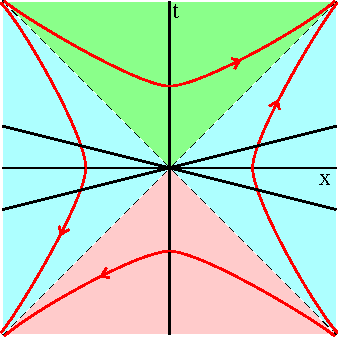
\includegraphics[scale=1]{boost}
				\caption{The \textbf{Rindler decomposition} of \textbf{Minkowski space}. The blue wedges are the Rindler wedges, the red one is the past wedge and the green one is the future wedge. The straight lines in black are slices of the Rindler time. The \textit{red lines} are the action of the \textit{boost operator} $K_x$.}\label{Rindler}
			\end{center}
		\end{figure}
	Now that we know  what entanglement is, we would also like to know, how much who is entangled with whom. In \textbf{Figure \ref{Rindler}} you can see a method which will help us, to reach that goal, the Rindler decomposition of Minkowski space.
	
	Therefore we split the Hilbert space into a factor $\Hil_L$ that acts on the fields $x<0$ and $\Hil_R$ for $x>0$. And each factor has its own basis of states with which we can decompose the vacuum.
	
	We now introduce the \textit{Lorentz boost\footnote{A Lorentz boost is a rotation-free Lorentz transformation, which is a Galilei-transformation in relativistic.\cite{ARTfliesbach} p.7} operator} $K_x$, which mixes x and t but does not act on the y or z direction. This operator exist in any relativistic QFT and looks in the free massive theory like this:
	\begin{equation}
		K_x = \frac{1}{2} \int \diff^3 x 
		\left[ x (\dot{\phi}^2 + \vec{\nabla} \phi \cdot \vec{\nabla} \phi + m^2 \phi^2) + t\dot{\phi} \partial_x \phi
		\right].
	\end{equation}
	It is not explicitly time-dependent, because if you plug it in Heisenberg's equation of motion the time-dependence of the fields cancels the explicit time dependence. \marginpar{Nachrechnen! (siehe QED übung)} In all four regions i.e. wedges of \textbf{Figure \ref{Rindler}} the action of $K_x$ is well defined. 
	
	So in the right blue wedge this operator is evolving forward in time, which is indicated by the red line with the arrow pointing in the increasing $t$ direction. On the contrary $K_x$ is evolving backwards in time in the left blue wedge, where the arrow on the red line is pointing at decreasing t direction. The upper and lower wedge are again the future and the past region where the action of $K_x$ is spacelike. 
	This figure looks very alike the Kruskal extension in \textbf{Figure \ref{kruskal}} but be careful and don't mix them up.
	\FloatBarrier